\documentclass[11pt,a4paper]{article}
\usepackage[margin=2.6cm]{geometry}
\usepackage{amsmath,amssymb}
\usepackage{booktabs,array}
\usepackage{enumitem}
\usepackage{xcolor}
\usepackage{graphicx}
\graphicspath{{../figs/}}
\usepackage{tikz}
\usepackage[colorlinks=true,linkcolor=teal!70!black,citecolor=teal!70!black,urlcolor=teal!70!black]{hyperref}

\definecolor{bandA}{HTML}{008A7C}
\definecolor{bandB}{HTML}{C2610C}

% Part I of the notebook draft (paper/draft-v6.tex), rewritten as a standalone methods note. Session 11, 2026-10-27.
% TODO (Roberto): author line and affiliation; AI-use statement wording; code URL; endorser.

\title{Geometry by counting in $1+1$ causal sets:\\ a rectangle identity, curvature from depth drift,\\ a calibrated embedding test, and a density-free propagator target}
\author{Roberto Bada\\ \small Independent researcher}  % TODO: confirm
\date{Draft v1, 27 October 2026}

\begin{document}
\maketitle

\begin{abstract}
In causal set theory spacetime is a locally finite partial order, and geometry must be read from the order alone. We collect and test a set of counting tools for $1+1$ dimensions. (i) For two spacelike events, the volumes of the causal-overlap regions of Bogu\~n\'a and Krioukov with respect to \emph{any} event $c$ in their common past obey an exact identity in flat $1+1$ spacetime, $d^2=2V_AV_B/V_C$; their equal-time construction is the special case $V_A=V_B$. With a simple Poisson bias correction the estimate has no measurable bias above two discreteness lengths and an error of 2--5\% at $10\ell$--$40\ell$. (ii) In curved spacetime the identity fails in a controlled way: the estimate depends on how deep $c$ lies. In de Sitter space the ratio is exactly $\tanh^2(H\tau/2)/[2\ln\cosh(H\tau/2)]=1-R\tau^2/16+\dots$ as $d\to0$, which turns the depth drift into a curvature estimator; it is unbiased on sprinklings but needs $\sim100$ pairs for $\pm20\%$ on $R$. (iii) Lorentzian multidimensional scaling of counted intervals, following Clough and Evans, recovers positions to half a discreteness length; we calibrate its spectral statistics against universe size and curvature, show that it misses layered orders because their sampled intervals are mostly of zero length, and add the share of zero-length pairs as the missing flag. On $e^{-\beta S}$ Monte Carlo universes at $N=200$ and $400$ the combined test separates the continuum-like and layered phases without error, including on held-out chains. (iv) For Johnston's chain-sum propagator, the mean over intervals with exactly $n$ elements in a random 2D order is $\tfrac12L_n(m^2/2\rho)$, a Laguerre polynomial; Johnston's continuum result is its Poisson average. This gives a target that needs no density, and it separates continuum-like universes from crystals. Everything here is $1+1$; we say which parts fail in higher dimensions.
\end{abstract}

\section{Introduction}
A causal set is a set of events with a partial order (``$x$ precedes $y$'') that is locally finite: every interval $I(x,y)=\{z:x\prec z\prec y\}$ is finite~\cite{BLMS87,Surya19}. The hypothesis of causal set theory is that spacetime is such a set, with the continuum a large-scale approximation. Order and number then carry all the geometry: the number of events in a region measures its volume, and the order fixes the light cones. The kinematic programme is to recover everything else from these two.

Some of this is classical. The longest chain between two events estimates their proper time~\cite{BrightwellGregory91}; interval and chain abundances give the dimension and curvature~\cite{RSS13,GlaserSurya13}; the Benincasa--Dowker operator gives the scalar curvature and the action~\cite{BD10,DowkerGlaser13}. Spatial distance is harder, because spacelike events have no interval between them. Bogu\~n\'a and Krioukov recently measured it through the overlap of the pasts of two events, seen from an event $c$ at equal proper time below both~\cite{BK24}; Hu, Meyer and Meyer gave an exact $1+1$ reconstruction from a past and a future event~\cite{HMM25}. Whether a given causal set looks like a manifold at all is tested by dimension estimators, interval abundances~\cite{GlaserSurya13} and Lorentzian embeddings~\cite{CloughEvans16,Henson06,Johnston25}. On the dynamical side, matter can be put on the order through Johnston's sum over chains~\cite{Johnston08,Johnston09}, whose average over sprinklings reproduces the Klein--Gordon propagator.

This note adds four small, checkable pieces in $1+1$ dimensions, and tests each on Poisson sprinklings against the known continuum:
\begin{enumerate}[leftmargin=*,itemsep=1pt]
\item a rectangle identity that frees the overlap distance from the equal-time choice of $c$ (Sec.~\ref{sec:dist});
\item curvature from the way that estimate drifts with the depth of $c$, with a closed form in de Sitter space (Sec.~\ref{sec:curv});
\item a calibration of the Lorentzian-embedding test against size and curvature, and a blind spot for layered orders with its fix (Sec.~\ref{sec:embed}), applied to classical growth and to the two phases of $e^{-\beta S}$ models (Sec.~\ref{sec:phases});
\item an exact, density-free target for Johnston's propagator at fixed interval size (Sec.~\ref{sec:prop}).
\end{enumerate}
None of these is deep; we think they are useful, and we did not find them in the literature (Sec.~\ref{sec:disc} lists what we checked). All code is available (see the end).

\section{Setting}\label{sec:setting}
We generate test universes by sprinkling: a Poisson process of density $\rho$ in a region of a known spacetime, with the order induced by the light cones. We then discard the coordinates and compare what the counting tools find with the truth. In $1+1$ dimensions we write $\ell=\rho^{-1/2}$ for the discreteness length: a patch of volume $\ell^2$ holds one event on average.

We use light-cone coordinates $u=t-x$, $v=t+x$, in which $dt\,dx=du\,dv/2$ and $x\prec y$ iff $u_x<u_y$ and $v_x<v_y$. The interval between $x\prec y$ is the rectangle $[u_x,u_y]\times[v_x,v_y]$, with volume $V=\Delta u\,\Delta v/2=\tau^2/2$. A sprinkled causal diamond is therefore a uniformly random \emph{2D order}: the intersection of two random linear orders~\cite{BHS08,Surya12}. For two spacelike events $d^2=\Delta x^2-\Delta t^2=-\Delta u\,\Delta v$.

Errors quoted are standard errors over independent sprinklings unless stated otherwise. The proper time from the longest chain has mean $\simeq2\sqrt n$ in an interval of $n$ events, with Tracy--Widom fluctuations of size $\simeq n^{1/6}$~\cite{BDJ99}; we use the count instead, $\tau^2=2n/\rho$, wherever a volume is available.

\section{Distance: a rectangle identity}\label{sec:dist}
Let $a,b$ be spacelike and $c$ an event in their common past. Following~\cite{BK24}, split the two intervals into
\begin{equation}
A=I(c,a)\setminus I(c,b),\qquad B=I(c,b)\setminus I(c,a),\qquad C=I(c,a)\cap I(c,b).
\end{equation}
Bogu\~n\'a and Krioukov choose $c$ at equal proper time $\tau_c$ below $a$ and $b$ and derive $d$ from the overlap fraction. In $1+1$ dimensions the choice of $c$ does not matter, because of the following identity (Fig.~\ref{fig:tiles}).

\begin{figure}[t]
\centering
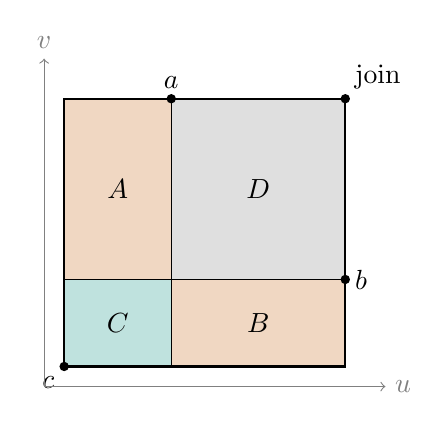
\begin{tikzpicture}[scale=0.85]
  \fill[bandA!25] (0,0) rectangle (1.6,1.3);
  \fill[bandB!25] (0,1.3) rectangle (1.6,4);
  \fill[bandB!25] (1.6,0) rectangle (4.2,1.3);
  \fill[gray!25] (1.6,1.3) rectangle (4.2,4);
  \draw[thick] (0,0) rectangle (4.2,4);
  \draw (1.6,0) -- (1.6,4); \draw (0,1.3) -- (4.2,1.3);
  \node at (0.8,0.65) {$C$}; \node at (0.8,2.65) {$A$}; \node at (2.9,0.65) {$B$}; \node at (2.9,2.65) {$D$};
  \fill (0,0) circle (2pt) node[below left] {$c$};
  \fill (1.6,4) circle (2pt) node[above] {$a$};
  \fill (4.2,1.3) circle (2pt) node[right] {$b$};
  \fill (4.2,4) circle (2pt) node[above right] {join};
  \draw[->,gray] (-0.3,-0.3) -- (4.8,-0.3) node[right] {$u$};
  \draw[->,gray] (-0.3,-0.3) -- (-0.3,4.6) node[above] {$v$};
\end{tikzpicture}
\caption{The rectangle identity in light-cone coordinates (rotate by $45^\circ$ for the usual picture). The rectangle from $c$ to the join of $a$ and $b$ splits into the overlap $C$, the strips $A$ and $B$ seen by only one of $a,b$, and the tile $D$ with $a$ and $b$ at opposite corners. Opposite tiles have equal products, $V_CV_D=V_AV_B$, and $V_D=d^2/2$.}
\label{fig:tiles}
\end{figure}

\paragraph{Derivation.} Put $c$ at the origin and take $u_a<u_b$, $v_a>v_b$ ($a$ and $b$ spacelike). Then $I(c,a)=[0,u_a]\times[0,v_a]$ and $I(c,b)=[0,u_b]\times[0,v_b]$. The rectangle from $c$ to the join $(u_b,v_a)$ splits into four tiles,
\begin{equation}
C=[0,u_a]\times[0,v_b],\quad A=[0,u_a]\times[v_b,v_a],\quad B=[u_a,u_b]\times[0,v_b],\quad D=[u_a,u_b]\times[v_b,v_a].
\end{equation}
With $\Delta u=u_b-u_a$ and $\Delta v=v_a-v_b$ the volumes are $V_C=u_av_b/2$, $V_A=u_a\Delta v/2$, $V_B=\Delta u\,v_b/2$, $V_D=\Delta u\,\Delta v/2$, so $V_CV_D=V_AV_B$. The tile $D$ has $a$ and $b$ at opposite corners, so $V_D=\Delta u\,\Delta v/2=d^2/2$. Hence, for every $c$ in the common past,
\begin{equation}
d^2=\frac{2V_AV_B}{V_C}.
\label{eq:rect}
\end{equation}
The equal-time choice of~\cite{BK24} is $V_A=V_B$, and their $1+1$ formula reduces to Eq.~\eqref{eq:rect} in that case. The identity uses that the overlap of two $1+1$ intervals is again an interval; in more dimensions it is not, and Eq.~\eqref{eq:rect} has no direct analogue.

\paragraph{Estimator.} On a causal set, $V_X$ is replaced by $N_X/\rho$, the number of events in the region. The three regions are disjoint, so $N_A$, $N_B$, $N_C$ are independent Poisson variables with means $\lambda_X=\rho V_X$. Then $N_AN_B$ is unbiased for $\lambda_A\lambda_B$, but $1/N_C$ is biased (and undefined at $N_C=0$). Since $E[1/(N+1)]=(1-e^{-\lambda})/\lambda$ for a Poisson variable,
\begin{equation}
\widehat{d^2}=\frac{2N_AN_B}{\rho\,(N_C+1)}
\label{eq:est}
\end{equation}
is unbiased up to $e^{-\lambda_C}$. Without the $+1$ a flat control read $11\%$ high at shallow $c$. The relative variance is about $1/\lambda_A+1/\lambda_B+1/\lambda_C$, so the deepest available $c$ is best. The strips $A$ and $B$ are long and thin, and hold many events even when $d\sim\ell$; this is why overlap estimators work down to the discreteness scale.

\paragraph{Test.} Table~\ref{tab:dist} and Fig.~\ref{fig:distance} use flat sprinklings in a unit diamond, random spacelike pairs among the late events, and for each pair the deepest $c$ (largest $N_C$). There is no measurable bias above $2\ell$, and the error at large $d$ falls roughly as $N^{-1/2}$. Below $2\ell$ the error stays near $20\%$ for all $N$: that is the discreteness scale itself.

\begin{table}[t]
\centering\small
\begin{tabular}{@{}rccc@{}}
\toprule
$N$ & $d<2\ell$ & $2\ell$--$10\ell$ & $>10\ell$\\
\midrule
1000 & 23\% & 6.5\% & 5.2\%\\
2000 & 15\% & 5.0\% & 3.4\%\\
4000 & 19\% & 5.1\% & 2.5\%\\
\bottomrule
\end{tabular}
\caption{Median relative error of Eq.~\eqref{eq:est} with the deepest $c$, flat $1+1$ sprinklings, 300 pairs $\times$ 4 sprinklings per $N$.}
\label{tab:dist}
\end{table}

\begin{figure}[t]
\centering
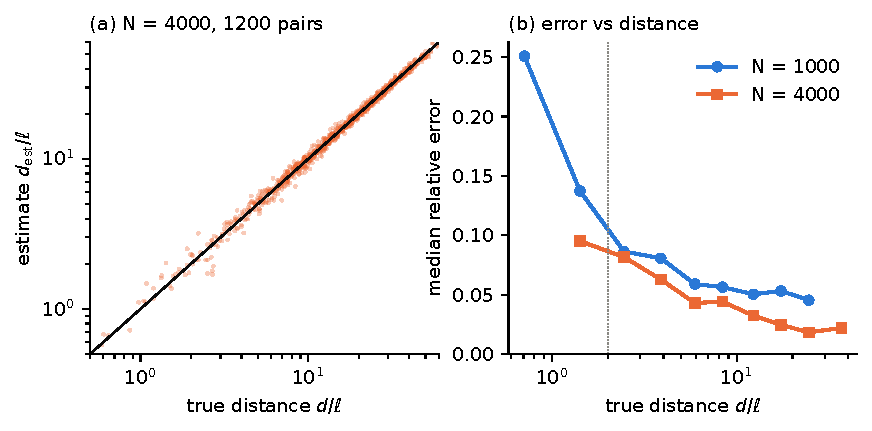
\includegraphics[width=0.92\linewidth]{fig_distance}
\caption{Eq.~\eqref{eq:est} with the deepest $c$ on flat $1+1$ sprinklings, from the causal order only. (a) Estimate against true distance, $N=4000$. (b) Median relative error per distance bin; the dotted line marks $2\ell$.}
\label{fig:distance}
\end{figure}

\section{Curvature from depth drift}\label{sec:curv}
In flat space every $c$ in the common past gives the same answer. In curved space Eq.~\eqref{eq:rect} is no longer exact, and the estimate depends on how deep $c$ lies. That dependence measures curvature.

\paragraph{de Sitter volumes.} Two-dimensional de Sitter space in conformal coordinates,
\[ds^2=\frac{-d\eta^2+dx^2}{(H\eta)^2},\qquad\eta<0,\]
has the same light cones as flat space. The tiles $A,B,C,D$ are the same rectangles in $(u,v)=(\eta-x,\eta+x)$, but volumes are weighted,
\[dV=\frac{d\eta\,dx}{(H\eta)^2}=\frac{2\,du\,dv}{H^2(u+v)^2}.\]
Integrating over $[u_1,u_2]\times[v_1,v_2]$, the inner integral gives $1/(u+v_1)-1/(u+v_2)$ and the outer one a logarithm:
\begin{equation}
V_\square=\frac{2}{H^2}\ln\frac{\eta_L\,\eta_R}{\eta_{\rm bot}\,\eta_{\rm top}},
\label{eq:dsvol}
\end{equation}
with $\eta=(u+v)/2$ evaluated at the left, right, bottom and top corners.

\paragraph{Closed form.} Put $a,b$ on one slice, $(\eta_0,\mp h)$, and $c$ straight below at $(\eta_0-T,0)$; set $H=1$. By symmetry $V_A=V_B$. From Eq.~\eqref{eq:dsvol}, to first order in $h$,
\begin{equation}
\begin{aligned}
V_A&=2\Big[\ln\big(q+\tfrac h2\big)+\ln(\eta_0-h)-\ln\big(q-\tfrac h2\big)-\ln\eta_0\Big]\\
&\simeq2h\Big(\frac1q-\frac1{\eta_0}\Big)=\frac{hT}{\eta_0\,q},\qquad q=\eta_0-\tfrac T2,
\end{aligned}
\end{equation}
and at $h=0$
\begin{equation}
V_C=2\ln\frac{q^2}{(\eta_0-T)\,\eta_0}=-2\ln(1-x),\qquad x=\frac{T^2}{4q^2}.
\end{equation}
The true distance is $d\simeq2h/|\eta_0|$. So
\begin{equation}
\frac{d^2_{\rm est}}{d^2}=\frac{2V_A^2/V_C}{4h^2/\eta_0^2}=\frac{x}{-\ln(1-x)}.
\end{equation}
The proper time from $c$ up to the midpoint of $a,b$ is $\tau=\ln(|\eta_0-T|/|\eta_0|)$, so $T/|\eta_0|=e^{\tau}-1$ and $x=\big((e^\tau-1)/(e^\tau+1)\big)^2=\tanh^2(\tau/2)$. Restoring $H$,
\begin{equation}
\frac{d^2_{\rm est}}{d^2}=\frac{\tanh^2(H\tau/2)}{2\ln\cosh(H\tau/2)}=1-\frac{(H\tau)^2}{8}+O(\tau^4)=1-\frac{R\,\tau^2}{16}+\dots,\qquad R=2H^2,
\label{eq:drift}
\end{equation}
exact as $d\to0$ at any depth, and independent of $\eta_0$ as it must be by the symmetry of de Sitter space. We checked Eq.~\eqref{eq:drift} against the exact volumes, Eq.~\eqref{eq:dsvol}, to $10^{-5}$ for $H\tau=0.1$--$3$. A sideways offset of $c$ changes it little, and a finite $d$ adds a roughly depth-independent shift. Every $1+1$ metric is conformally flat, so the leading term should hold locally in any $1+1$ spacetime. We checked this beyond de Sitter in $1+1$ FRW spacetimes $ds^2=a(\eta)^2(-d\eta^2+dx^2)$ with $a=\eta^p$, where $R=2(\ln a)''/a^2=-2p\,\eta^{-2-2p}$ varies in time and the rectangle volumes have a closed form. For $p=1$, $-2$ and $\tfrac12$ (negative, positive and negative curvature), $16(1-d^2_{\rm est}/d^2)/\tau^2$ tends to $R$ at the location of $a,b$ as $\tau\to0$ (to $1\%$ at $\tau=0.01$), with the right sign: for $R<0$ the ratio rises above $1$. At finite depth it reads a curvature between the one at $a,b$ and the one at the proper-time midpoint: the drift averages $R$ over the region, weighted towards the top.

\paragraph{Test on sprinklings.} We sprinkle de Sitter ($H=1$, $\rho=10^4$) and, as a control, flat space in the same coordinates, insert $a,b$ by hand $\approx14\ell$ apart, and evaluate Eq.~\eqref{eq:est} for every sprinkled $c$ in their common past whose rectangle lies inside the region. Figure~\ref{fig:drift} shows the mean ratio per depth bin over 400 sprinklings against the continuum computed for the same $c$'s. The flat control stays at $1$ and de Sitter follows the continuum. Two cautions: neighbouring depth bins share events and are $\approx0.9$ correlated, so a run of deviations in adjacent bins is one fluctuation, not several (we saw a 2$\sigma$ run in a first batch of 100 sprinklings that disappeared in the next 300); and in the shallowest bin the tiles hold few events and the estimator reads low in both geometries.

\begin{figure}[t]
\centering
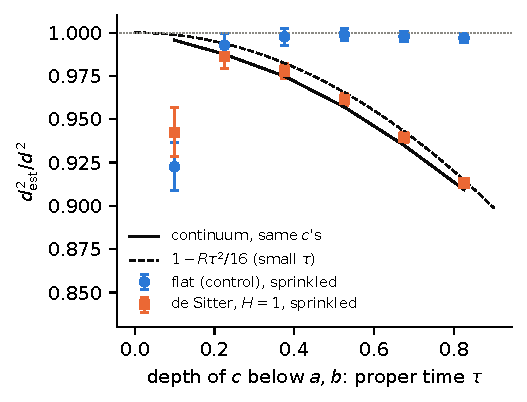
\includegraphics[width=0.52\linewidth]{fig_drift}
\caption{Depth drift of the rectangle estimate. Mean over 400 sprinklings ($\rho=10^4$) per bin of the proper time $\tau$ from $c$ up to $a,b$; errors from the spread between sprinklings. Solid: continuum ratio from the exact volumes, averaged over the same $c$'s. Dashed: the small-$\tau$ term of Eq.~\eqref{eq:drift}.}
\label{fig:drift}
\end{figure}

\paragraph{A curvature estimator.} Using only counts, fit $\widehat{d^2}=\alpha+\beta\tau^2$ over the $c$'s of one pair with $\tau\in[0.2,0.7]$ and $\tau^2=(N_{I(c,a)}+N_{I(c,b)})/\rho$, and set $R_{\rm est}=-16\beta/\alpha$. Over 100 sprinklings, one pair each:
\begin{center}\small
\begin{tabular}{@{}rccc@{}}
\toprule
$\rho$ & flat (true $R=0$) & de Sitter (true $R=2$; continuum fit $1.9$--$2.2$) & spread per pair\\
\midrule
4000 & $-0.7\pm0.6$ & $1.3\pm0.7$ & $\approx6$--$7$\\
$10^4$ & $0.3\pm0.4$ & $1.6\pm0.4$ & $\approx4$\\
\bottomrule
\end{tabular}
\end{center}
The continuum value depends on whether $\tau$ is the true proper time ($1.88$) or read from interval volumes as the counts do ($2.2$). In the $p=1$ FRW spacetime above ($\rho=10^4$, 200 sprinklings, $a,b$ at $\eta_0=1.5$), the binned ratio follows the exact continuum within $1\sigma$ for $\tau\ge0.15$, and the fit gives $R_{\rm est}=-1.25\pm0.30$ against $-0.81$ for the same fit on the continuum, while $R$ itself runs from $-0.4$ at $a,b$ to $-2.8$ at the bottom of the window. The fit therefore measures a depth-weighted average of $R$, not $R$ at $a,b$. The estimator is right on average and tells flat from curved, but a single pair is useless: about 100 pairs are needed for $\pm0.4$. That is comparable in spirit to other counting routes to curvature, through the Benincasa--Dowker operator~\cite{BD10}, chain abundances~\cite{RSS13} or Ollivier--Ricci curvature~\cite{BBR26}. Its advantage is geometric transparency: the curvature is the failure of one exact flat-space identity, read off as a function of depth. Bogu\~n\'a and Krioukov remark that their method extends locally to curved spacetimes~\cite{BK24}; we did not find a curvature estimator built from it among the papers that cite them.

\section{Shape: an embedding test and its blind spot}\label{sec:embed}
\paragraph{Embedding.} Given the squared intervals $s_{ij}$ between $M$ sampled events, classical multidimensional scaling (MDS) with a Lorentzian Gram matrix reconstructs coordinates. Clough and Evans applied it to causal sets and proposed its eigenvalue spectrum as a test of dimension and manifoldness~\cite{CloughEvans16}. With $s_{ij}=(x_i-x_j)^{\!\top}\eta\,(x_i-x_j)$, double centring, $G=-\tfrac12JSJ$ with $J=I-\mathbf1\mathbf1^{\!\top}/M$, gives $G=X\eta X^{\!\top}$ for the centred coordinates $X$. A $1+1$ Lorentzian set shows one large negative eigenvalue (time), one large positive one (space) and the rest near zero; the two eigenvectors give coordinates up to a Lorentz transformation.

We feed MDS with counts only: $s=-2N(I)/\rho$ for related pairs and Eq.~\eqref{eq:est} with the deepest $c$ for spacelike pairs. On $M=150$ events of a flat sprinkling with $N=2000$, positions are recovered to $0.43\pm0.07\,\ell$ across a region $\approx38\ell$ wide; the map to the true coordinates is a Lorentz transformation to within 3--10\%; and the spectrum is $\lambda_-\approx-2.2$, $\lambda_+\approx2.2$, all others below $0.1$. A $2+1$ sprinkling fed through the same pipeline shows two large positive eigenvalues, so the spectrum counts spatial dimensions even though Eq.~\eqref{eq:est} is a $1+1$ formula.

\paragraph{Statistics and calibration.} As a test we use intrinsic numbers only: $r_+$, the ratio of the second to the first positive eigenvalue; and the \emph{stress}, the rms misfit of the squared intervals by the best $1+1$ Minkowski embedding, relative to their rms. The sample is the $M=40$ events with the largest pasts (after removing events without a common past with the rest). Fig.~\ref{fig:detector}a shows the calibration on flat universes (random 2D orders): stress and $r_+$ settle only for $N\gtrsim100$ (stress $0.16$, $0.10$, $0.08$ at $N=100$, $200$, $400$); below $N\approx50$ a flat universe looks as bad as a crystal. Curvature raises the stress: on de Sitter diamonds of fixed $N=400$ it stays in the flat band up to $H\tau\approx1$ and reaches $0.25$ at $H\tau=4$ (Fig.~\ref{fig:detector}c). The stress therefore answers ``is it a \emph{flat} sheet?'', while Sec.~\ref{sec:curv} measures how curved it is.

\paragraph{Blind spot.} Applied to $e^{-\beta S}$ Monte Carlo universes at $N=400$ (Sec.~\ref{sec:phases}), this test passes every continuum-like state and fails 4- and 7-layer orders, but it does not reliably flag orders with $\sim10$ layers: at $M=40$ one of seven sits in the flat band and two more just above it, and at $M=80$ two others read stress $0.03$, \emph{better} than flat. Two things go wrong. The sample sees only the top layer or two. And in a layered order most sampled pairs have zero squared interval: linked pairs have $N(I)=0$, and spacelike pairs often have an empty strip, $N_A=0$ or $N_B=0$. MDS fits an all-zero matrix perfectly; a bilayer gives exactly that.

\paragraph{The fix.} We add a second number, the share $z$ of sampled pairs with zero squared interval, taken as the larger of its values on the top sample and on a sample spread evenly in height (longest chain below the event) over the upper $70\%$ of the order. On sprinklings $z$ falls with $N$ (median $0.18$, $0.12$, $0.09$ at $N=100$, $200$, $400$) and does not respond to curvature: de Sitter diamonds at $H\tau=4$ read $0.08$--$0.11$. Layered orders read $0.4$--$1$ (Fig.~\ref{fig:detector}b). We flag a universe as layered when $z>1.5\times$ the flat median at the same $N$. The share of zero-length pairs is a cousin of the interval-abundance tests of Glaser and Surya~\cite{GlaserSurya13}; what we add is that the embedding test needs it, and its calibration. The combined test asks two questions: \emph{is it layered?} ($z$) and \emph{is it a flat sheet?} (stress). Orders with only 2--3 layers break the pipeline (too few events have a common past), which we count as a failure.

\begin{figure}[t]
\centering
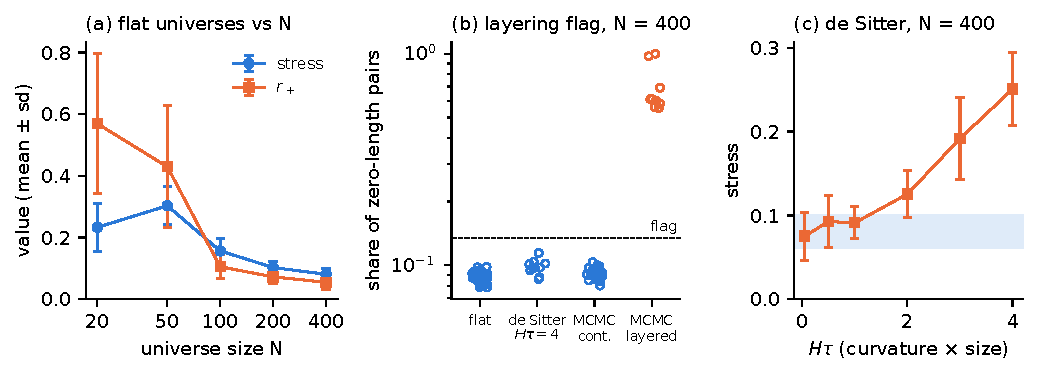
\includegraphics[width=\linewidth]{fig_detector}
\caption{Calibrating the embedding test. (a) Flat universes (random 2D orders, 10 per size, $M=40$): stress and $r_+$ against $N$. (b) Share of zero-length pairs at $N=400$ ($M=80$): flat universes, de Sitter diamonds at $H\tau=4$, and final states of $e^{-\beta S}$ Monte Carlo chains (continuum-like, 30--39 layers; layered, 4--11 layers). Dashed: the flag, $1.5\times$ the flat median. The 13 states with 2--3 layers are not shown. (c) Stress of de Sitter diamonds at fixed $N=400$ (8 per height) against $H\tau$; shaded: the flat band ($\pm1$ sd).}
\label{fig:detector}
\end{figure}

\section{Which 2D orders look like spacetime?}\label{sec:phases}
\paragraph{Classical growth.} In classical sequential growth~\cite{RideoutSorkin00} events are born one at a time and each newborn picks its past among existing events. We grew $N=100$ universes with a fixed link probability $p=0.05$ and with $p_n=3/n$ (an expanding universe from a single first event). Neither gives a $1+1$ spacetime: the ordering-fraction (Myrheim--Meyer) dimension drifts with scale, and the embedding test fails on every number (share of the spectrum in one time and one space direction $\approx0.33$ against $0.65$ for flat universes of the same size, stress $\approx0.65$ against $0.19$). At $N=200$ they still fail on stress ($0.64$--$0.78$ against $\approx0.12$ for flat universes); their zero share is not what flags them. The second rule also uses the birth order as a clock; covariant routes to cosmology in growth models are discussed in~\cite{MORS01,AhmedRideout10}.

\paragraph{The two phases of $e^{-\beta S}$.} Weighting 2D orders by $e^{-\beta S}$, with $S$ the Benincasa--Dowker action, gives a first-order transition between a continuum-like phase and a layered phase~\cite{BHS08,Surya12,GOS18}. We sampled it with Metropolis swap moves at non-locality parameter $\epsilon=0.21$ (an $O(N^2)$ update: a swap changes two rows and columns of the causal matrix). At $N=200$ the test gives:
\begin{center}\small
\begin{tabular}{@{}lccccc@{}}
\toprule
$N=200$ & ordering fraction & layers & $r_+$ & stress & zero share $z$ (fresh chains)\\
\midrule
flat (random orders) & 0.50 & 24 & 0.07 & 0.10 & 0.10--0.15\\
$\beta=0.05$ (continuum-like) & 0.51 & 24 & 0.10 & 0.11 & 0.12--0.13 ($\beta\le0.3$)\\
$\beta=0.6$ (layered) & 0.59 & 9 & 0.39 & 0.28 & 0.39--0.48 ($\beta\ge0.6$, 8--13 layers)\\
\bottomrule
\end{tabular}
\end{center}
(The $\beta\ge0.6$ states are metastable intermediates; the known ground state at large $\beta$ is a bilayer~\cite{CunninghamSurya19}.) We then applied the flag of Sec.~\ref{sec:embed} to 44 final states of $N=400$ chains run from random and from layered starts at $0.01\le\beta\le0.7$. All 22 continuum-like states (30--39 layers) pass; all 9 states with 4--11 layers are flagged ($z=0.55$--$1.0$ against a threshold $0.13$); the 13 states with 2--3 layers break the pipeline. Because the rule was designed after seeing these states, we tested it on fresh $N=200$ chains: 12 of 12 continuum-like states passed and 18 of 18 layered states ($\beta=0.6$--$1.5$) were flagged. These states are test inputs, not equilibrium samples: the chains from layered starts accept $\le0.1\%$ of moves, so we do not use them to locate the transition. Our bracket $0.05<\beta_c(400)<0.45$ is consistent with the finite-size fit $\beta_c\approx1.66/(\epsilon^2N)=0.094$ of~\cite{GOS18}.

\section{A density-free target for Johnston's propagator}\label{sec:prop}
\paragraph{The propagator.} Johnston's particle hops along the order with amplitude $a$ per hop and $b$ per intermediate stop~\cite{Johnston08}. With $C$ the causal matrix ($C_{xy}=1$ if $x\prec y$) and $\Phi=aC$,
\begin{equation}
K=\Phi+b\,\Phi^2+b^2\Phi^3+\dots=\Phi\,(I-b\Phi)^{-1},\qquad a=\tfrac12,\quad b=-m^2/\rho\quad(1+1).
\end{equation}
$K(x,y)$ is a weighted count of chains: $K(x,y)=\tfrac12\sum_k c_k(x,y)\,(-\mu/2)^k$, with $c_k$ the number of $k$-element chains strictly inside $I(x,y)$ and $\mu=m^2/\rho$. In a sprinkled interval of volume $V=\tau^2/2$ the expected number of $k$-chains is $(\rho V)^k/(k!)^2$, so $\langle K\rangle=\tfrac12\sum_k\big(-(m\tau/2)^2\big)^k/(k!)^2=\tfrac12J_0(m\tau)$, the retarded Klein--Gordon propagator~\cite{Johnston08}.

\paragraph{Fixed interval size.} $K$ depends on the order and on $\mu$ only. In a uniformly random 2D order the $n$ events inside an interval form again a uniformly random 2D order, and any $k$ of them form a chain with probability $1/k!$ (the two linear orders must agree on them). So $E[c_k\,|\,n]=\binom nk/k!$~\cite{Pinsky06}, and
\begin{equation}
E[K\,|\,n]=\frac12\sum_{k=0}^n\binom nk\frac{(-\mu/2)^k}{k!}=\frac12L_n\!\Big(\frac\mu2\Big)\;\approx\;\frac12e^{\mu/4}J_0\Big(\sqrt{2\mu(n+\tfrac12)}\Big),
\label{eq:lag}
\end{equation}
a Laguerre polynomial in the interval size. Averaging over Poisson $n$ with mean $\lambda=\rho\tau^2/2$, $\sum_ne^{-\lambda}\frac{\lambda^n}{n!}\binom nk=\frac{\lambda^k}{k!}$, gives back $\tfrac12\sum_k(-\mu\lambda/2)^k/(k!)^2=\tfrac12J_0(m\tau)$: Johnston's result is the Poisson average of Eq.~\eqref{eq:lag}. The fixed-$n$ form needs no density and no coordinates: every related pair of a causal set supplies its $n$ and its $K$, and Eq.~\eqref{eq:lag} is the target. The identity itself is combinatorics: at $\mu=-2$ and summed over permutations it counts all increasing subsequences, $n!\,L_n(-1)$ (OEIS A002720; ~\cite{LifschitzPittel81}). We did not find its application to the propagator among the 99 papers on arXiv citing~\cite{Johnston08,Johnston09}; later path-sum work averages over sprinklings~\cite{Shuman23,KastratiHinrichsen26}. Expanding in $\mu$, the first term that can fail is the ordering fraction, i.e.\ the Myrheim--Meyer dimension, so the propagator is a resummed tower of dimension tests.

\paragraph{Tests.} Figure~\ref{fig:laguerre} bins all related pairs of an $N=400$ universe by $n$ and compares $\langle K\rangle$ with Eq.~\eqref{eq:lag} at $\mu=0.05$. A random order and continuum-like $e^{-\beta S}$ universes follow the target (rms deviation $0.012$--$0.020$ over all pairs, the same as for random controls, $0.014$--$0.017$). Layered states with $\sim10$ layers deviate with rms $0.07$--$0.10$, five times more, so the propagator also flags the states that the unpatched embedding test missed (Sec.~\ref{sec:embed}). Crystals fail: in a 4-layer order no interval holds more than 9 events, so $K$ never turns negative and the mass never shows; a 7-layer order falls below the target (too many chains). Classically grown universes ($N=1500$) fail systematically, one ($p=0.02$) reaching $|K|\approx10$, far beyond the $1+1$ bound $\tfrac12$.

\paragraph{Curvature at fixed $n$.} In curved $1+1$ spacetime a term $(R\tau^2/48)J_2(m\tau)$ appears~\cite{NXDS17}. In a de Sitter diamond conditioned on $n$ events the order depends only on $(n,H\tau)$, so a fixed-$n$ curvature test exists. We find that the share of related pairs rises by $\approx0.027\,(H\tau)^2$ for $n=10$--$60$, and that the fixed-$n$ propagator is no more sensitive than that share alone (a $3\sigma$ detection at $n=30$, $H\tau=1$ needs 175 intervals either way). The fixed-$n$ propagator thus sees curvature through the known chain-abundance route~\cite{RSS13}; we record this as a negative result.

\begin{figure}[t]
\centering
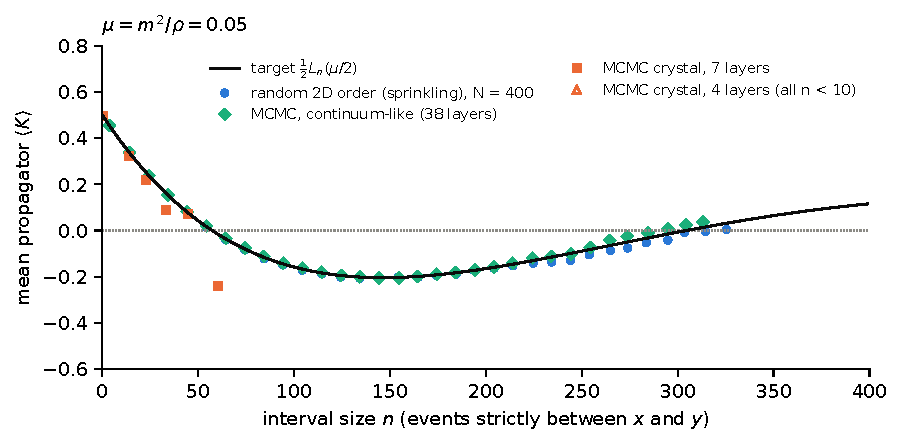
\includegraphics[width=0.92\linewidth]{fig_laguerre}
\caption{Johnston's propagator averaged over related pairs with interval size $n$, against $\tfrac12L_n(\mu/2)$, at $\mu=0.05$ and $N=400$. At large $n$ few pairs remain and the bins are noisy. In the 4-layer crystal every interval has fewer than 10 events, so it contributes a single point near $n=0$.}
\label{fig:laguerre}
\end{figure}

\section{Discussion}\label{sec:disc}
\paragraph{What is new, and what we checked.} The overlap regions are from~\cite{BK24} and the embedding from~\cite{CloughEvans16}; the zero-share flag is a relative of~\cite{GlaserSurya13}, and the Laguerre identity is classical combinatorics. To our knowledge the following are new: the general-$c$ rectangle identity, Eq.~\eqref{eq:rect}, with the bias-corrected estimator; the depth-drift curvature estimator and its closed form, Eq.~\eqref{eq:drift}; the calibration of the embedding test against size, curvature and layering; and the fixed-$n$ target, Eq.~\eqref{eq:lag}. For each we read the full citation lists of the closest papers (\cite{BK24}, \cite{CloughEvans16}, \cite{Johnston08,Johnston09}) and searched the full texts; the rectangle identity is elementary enough that it may appear in passing somewhere we did not look.

\paragraph{Limitations.} Everything quantitative is $1+1$. The rectangle identity has no direct analogue in higher dimensions, where the overlap of two intervals is not an interval; the absence of a robust spatial distance for $d>2$ is a known open problem~\cite{Surya19}. The curvature estimator is noisy (about 100 pairs for $\pm20\%$) and was tested on de Sitter and one FRW spacetime; it measures a depth-weighted average of $R$. The embedding thresholds are empirical and must be recalibrated at each $N$; the $e^{-\beta S}$ states we used are test inputs, not equilibrium samples. The Laguerre target is exact only for 2D orders.

\paragraph{Outlook.} Two extensions look natural: a version of the depth drift built from Hu--Meyer--Meyer's past-and-future construction~\cite{HMM25}, which may be less noisy, and a fixed-$n$ target in $3+1$. There the exactness of Eq.~\eqref{eq:lag} is lost: Johnston's $3+1$ particle hops along links only~\cite{Johnston08}, so a path requires every skipped sub-interval to be empty, and $E[K\,|\,n]$ becomes a sum of $(k-1)$-point integrals with factors $(1-W/V)^{n-k+1}$. Its first term can be done for large $n$: the expected number of two-hop link paths tends to $3\pi$, which reproduces exactly the short-distance limit $m^2/8\pi$ of the continuum mass term; a Monte Carlo check approaches it as $3\pi(1-1.6/\sqrt n)$. A $3+1$ target is therefore a computed table rather than a formula.

\section*{Code and data}
All simulations are short numpy scripts; the figures are produced by \texttt{sims/fig\_part1.py}, the detector fix by \texttt{sims/r8\_detector\_spread.py}, the curvature fit and the FRW check by \texttt{sims/r9\_drift\_fit\_frw.py}, and the $N=400$ Monte Carlo states by \texttt{sims/n400\_crystal.py}. Repository: \textit{[URL to be added]}.

\section*{Acknowledgements and use of AI tools}
% TODO (Roberto): wording. arXiv policy: AI tools cannot be authors; their use must be disclosed.
The author used Claude (Anthropic), an AI system, as a research assistant: for literature searches, for checking derivations, for writing simulation code and for drafting text. All results were checked by running the code; the author takes full responsibility for the content.

\begin{thebibliography}{99}\small
\bibitem{BLMS87} L.~Bombelli, J.~Lee, D.~Meyer, R.~D.~Sorkin, ``Space-time as a causal set'', Phys.\ Rev.\ Lett.\ 59, 521 (1987).
\bibitem{Surya19} S.~Surya, ``The causal set approach to quantum gravity'', Living Rev.\ Rel.\ 22, 5 (2019), arXiv:1903.11544.
\bibitem{BrightwellGregory91} G.~Brightwell, R.~Gregory, ``Structure of random discrete spacetime'', Phys.\ Rev.\ Lett.\ 66, 260 (1991).
\bibitem{RSS13} M.~Roy, D.~Sinha, S.~Surya, ``The discrete geometry of a small causal diamond'', Phys.\ Rev.\ D 87, 044046 (2013), arXiv:1212.0631.
\bibitem{GlaserSurya13} L.~Glaser, S.~Surya, ``Towards a definition of locality in a manifoldlike causal set'', Phys.\ Rev.\ D 88, 124026 (2013), arXiv:1309.3403.
\bibitem{BD10} D.~M.~T.~Benincasa, F.~Dowker, ``The scalar curvature of a causal set'', Phys.\ Rev.\ Lett.\ 104, 181301 (2010).
\bibitem{DowkerGlaser13} F.~Dowker, L.~Glaser, ``Causal set d'Alembertians for various dimensions'', arXiv:1305.2588.
\bibitem{BK24} M.~Bogu\~n\'a, D.~Krioukov, ``Measuring spatial distances in causal sets via causal overlaps'', Phys.\ Rev.\ D 110, 024008 (2024), arXiv:2401.17376.
\bibitem{HMM25} C.~A.~Hu, D.~A.~Meyer, E.~J.~Q.~Meyer, ``Reconstructing Minkowski geometry from causal separations'', J.\ Math.\ Phys.\ 66, 122502 (2025), arXiv:2601.03280.
\bibitem{CloughEvans16} J.~R.~Clough, T.~S.~Evans, ``Embedding graphs in Lorentzian spacetime'', PLoS ONE 12, e0187301 (2017), arXiv:1602.03103.
\bibitem{Henson06} J.~Henson, ``Constructing an interval of Minkowski space from a causal set'', Class.\ Quant.\ Grav.\ 23, L29 (2006), gr-qc/0601069.
\bibitem{Johnston25} S.~Johnston, ``Simpler embeddings of causal sets into Minkowski spacetime'', arXiv:2502.09701.
\bibitem{Johnston08} S.~Johnston, ``Particle propagators on discrete spacetime'', Class.\ Quant.\ Grav.\ 25, 202001 (2008), arXiv:0806.3083.
\bibitem{Johnston09} S.~Johnston, ``Feynman propagator for a free scalar field on a causal set'', Phys.\ Rev.\ Lett.\ 103, 180401 (2009), arXiv:0909.0944.
\bibitem{BHS08} G.~Brightwell, J.~Henson, S.~Surya, ``A 2D model of causal set quantum gravity: the emergence of the continuum'', Class.\ Quant.\ Grav.\ 25, 105025 (2008), arXiv:0706.0375.
\bibitem{Surya12} S.~Surya, ``Evidence for a phase transition in 2D causal set quantum gravity'', arXiv:1110.6244.
\bibitem{BDJ99} J.~Baik, P.~Deift, K.~Johansson, ``On the distribution of the length of the longest increasing subsequence of random permutations'', J.\ Amer.\ Math.\ Soc.\ 12, 1119 (1999).
\bibitem{BBR26} J.~Barton, S.~Borza, J.~R\"ohrig, ``Ollivier--Ricci curvature for causal sets'', arXiv:2606.04910 (2026).
\bibitem{RideoutSorkin00} D.~P.~Rideout, R.~D.~Sorkin, ``A classical sequential growth dynamics for causal sets'', Phys.\ Rev.\ D 61, 024002 (2000).
\bibitem{MORS01} X.~Mart\'in, D.~O'Connor, D.~P.~Rideout, R.~D.~Sorkin, ``On the renormalization transformations induced by cycles of expansion and contraction in causal set cosmology'', Phys.\ Rev.\ D 63, 084026 (2001).
\bibitem{AhmedRideout10} M.~Ahmed, D.~Rideout, ``Indications of de Sitter spacetime from classical sequential growth dynamics of causal sets'', Phys.\ Rev.\ D 81, 083528 (2010).
\bibitem{GOS18} L.~Glaser, D.~O'Connor, S.~Surya, ``Finite size scaling in 2d causal set quantum gravity'', Class.\ Quant.\ Grav.\ (2018), arXiv:1706.06432.
\bibitem{CunninghamSurya19} W.~J.~Cunningham, S.~Surya, ``Dimensionally restricted causal set quantum gravity: examples in two and three dimensions'', arXiv:1908.11647.
\bibitem{Pinsky06} R.~G.~Pinsky, ``Law of large numbers for increasing subsequences of random permutations'', arXiv:math/0407353, eq.~(1.1).
\bibitem{LifschitzPittel81} V.~Lifschitz, B.~Pittel, ``The number of increasing subsequences of the random permutation'', J.\ Combin.\ Theory A 31, 1 (1981) (not read by us; cited via OEIS A002720).
\bibitem{Shuman23} S.~Shuman, ``Path sums for propagators in causal sets'', arXiv:2307.08864.
\bibitem{KastratiHinrichsen26} A.~Kastrati, H.~Hinrichsen, ``Numerical evaluation of the causal set propagator in 2D anti-de Sitter spacetime'', Phys.\ Rev.\ D 113, 065003 (2026), arXiv:2504.12919.
\bibitem{NXDS17} Nomaan~X, F.~Dowker, S.~Surya, ``Scalar field Green functions on causal sets'', Class.\ Quant.\ Grav.\ 34, 124002 (2017), arXiv:1701.07212.
\end{thebibliography}
\end{document}
